\documentclass[11pt, a4paper]{article}
\usepackage[UTF8, heading=true]{ctex}
\usepackage[dvipsnames, x11names]{xcolor}
\usepackage{geometry}
\usepackage{subcaption}
\usepackage{float}
\usepackage{graphicx}
\usepackage{listings}

\newfontfamily\codefont{Cascadia Code}
\definecolor{codebackground}{RGB}{230 235 245}

\lstset{
    basicstyle          =   \small\codefont,
    % ---
    tabsize             =   4,
    showstringspaces    =   false,
    numbers             =   left,
    numberstyle         =   \codefont,
    % ---
    breaklines          =   true,
    captionpos          =   t,      
    % ---
    frame               =   l,
    flexiblecolumns,
}

\lstset{
    basicstyle          =   \small\codefont,
    % ---
    tabsize             =   4,
    showstringspaces    =   false,
    numbers             =   left,
    numberstyle         =   \codefont,
    % ---
    breaklines          =   true,
    captionpos          =   t,      
    % ---
    frame               =   l,
    flexiblecolumns,
    columns = fixed,
    % ---
    backgroundcolor     =   \color{codebackground},
}

\lstdefinestyle{python}{
    language        =   Python, % 语言选Python
    keywordstyle    =   \bfseries\color{blue},
    % keywordstyle    =   [2] \color{teal},
    stringstyle     =   \color{orange!80!black},
    commentstyle    =   \color{OliveGreen},
    % identifierstyle =   \color{blue!80!white},
    backgroundcolor =   \color{codebackground}
}
\lstMakeShortInline|

\geometry{a4paper, scale=0.8}

\ctexset{
    section = {
        name = {Task },
        format = {\Large\bfseries}
    }
}

\title{\Large{\bf{视听信息系统导论编程3}}}
\author{高艺轩\ 毕嘉仪}
\date{}

\begin{document}
\maketitle
\section{数据准备}
函数|prepare_data|首先将全部文本读入,根据要求进行数据预处理,然后给每一个单独的字符都赋予一个index并将所有字符、index对存储为字典类型,得到对应词表。

\section{完成dataset}

\section{无pos enc、无attn mask的Transformer}
训练结果:\begin{figure}[H]
    \hfill
    \begin{subfigure}[t]{0.45\linewidth}
        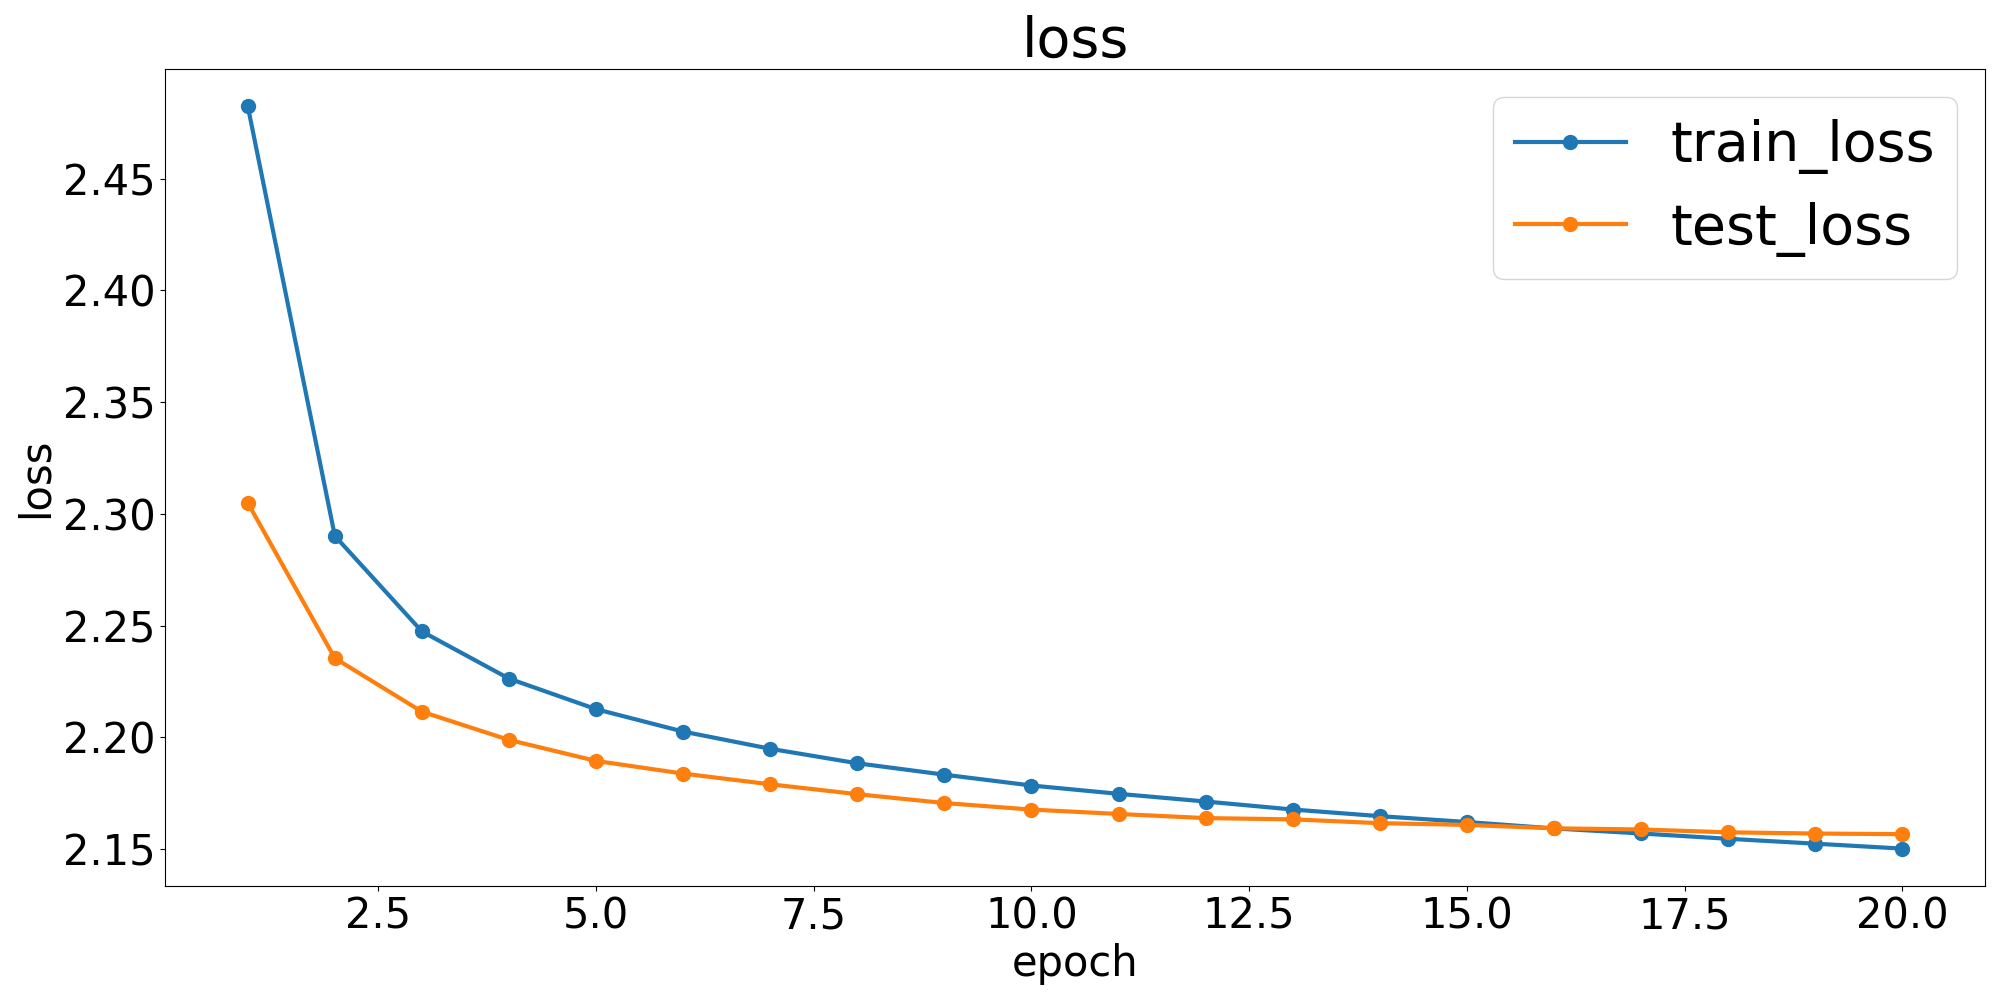
\includegraphics[width=\textwidth]{img/3-1.png}
    \end{subfigure}
    \hfill
    \begin{subfigure}[t]{0.45\linewidth}
        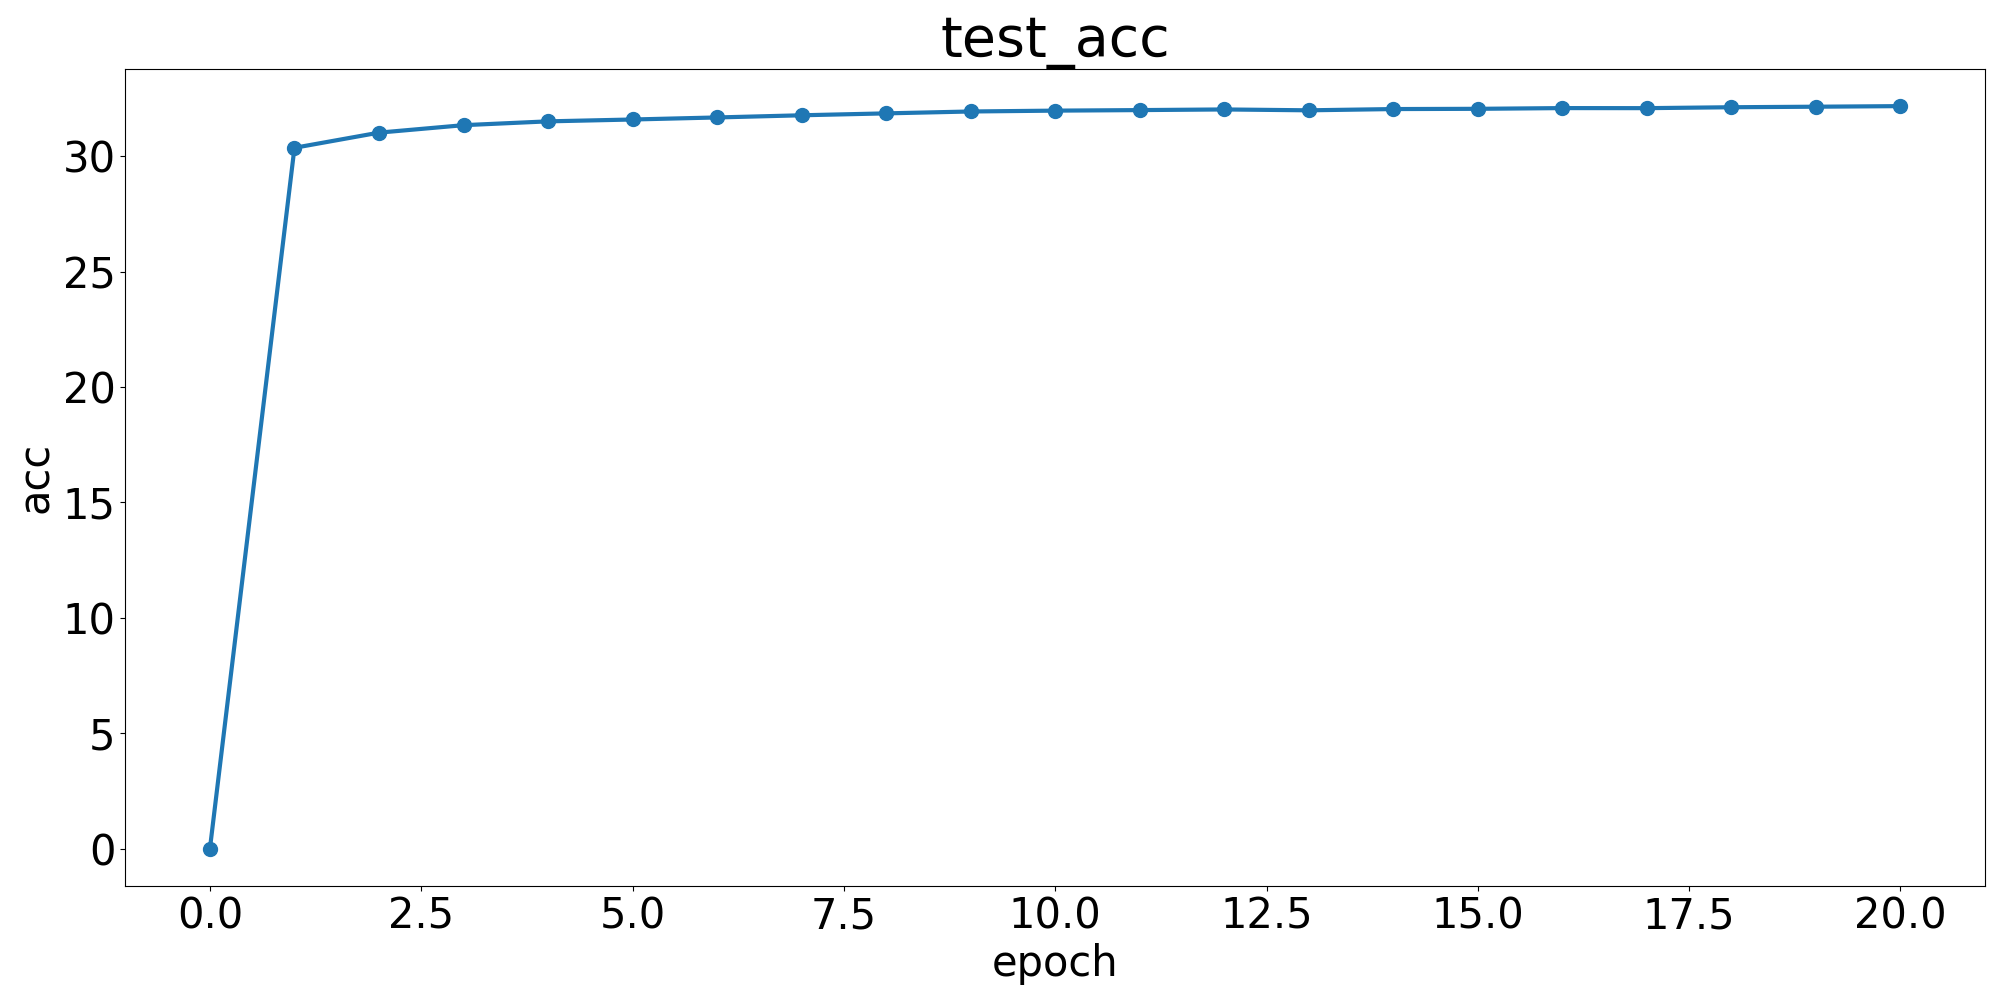
\includegraphics[width=\textwidth]{img/3-2.png}
    \end{subfigure}
    \hfill
\end{figure}


\section{有pos enc、无attn mask的Transformer}
训练结果:
\begin{figure}[H]
    \hfill
    \begin{subfigure}[t]{0.45\linewidth}
        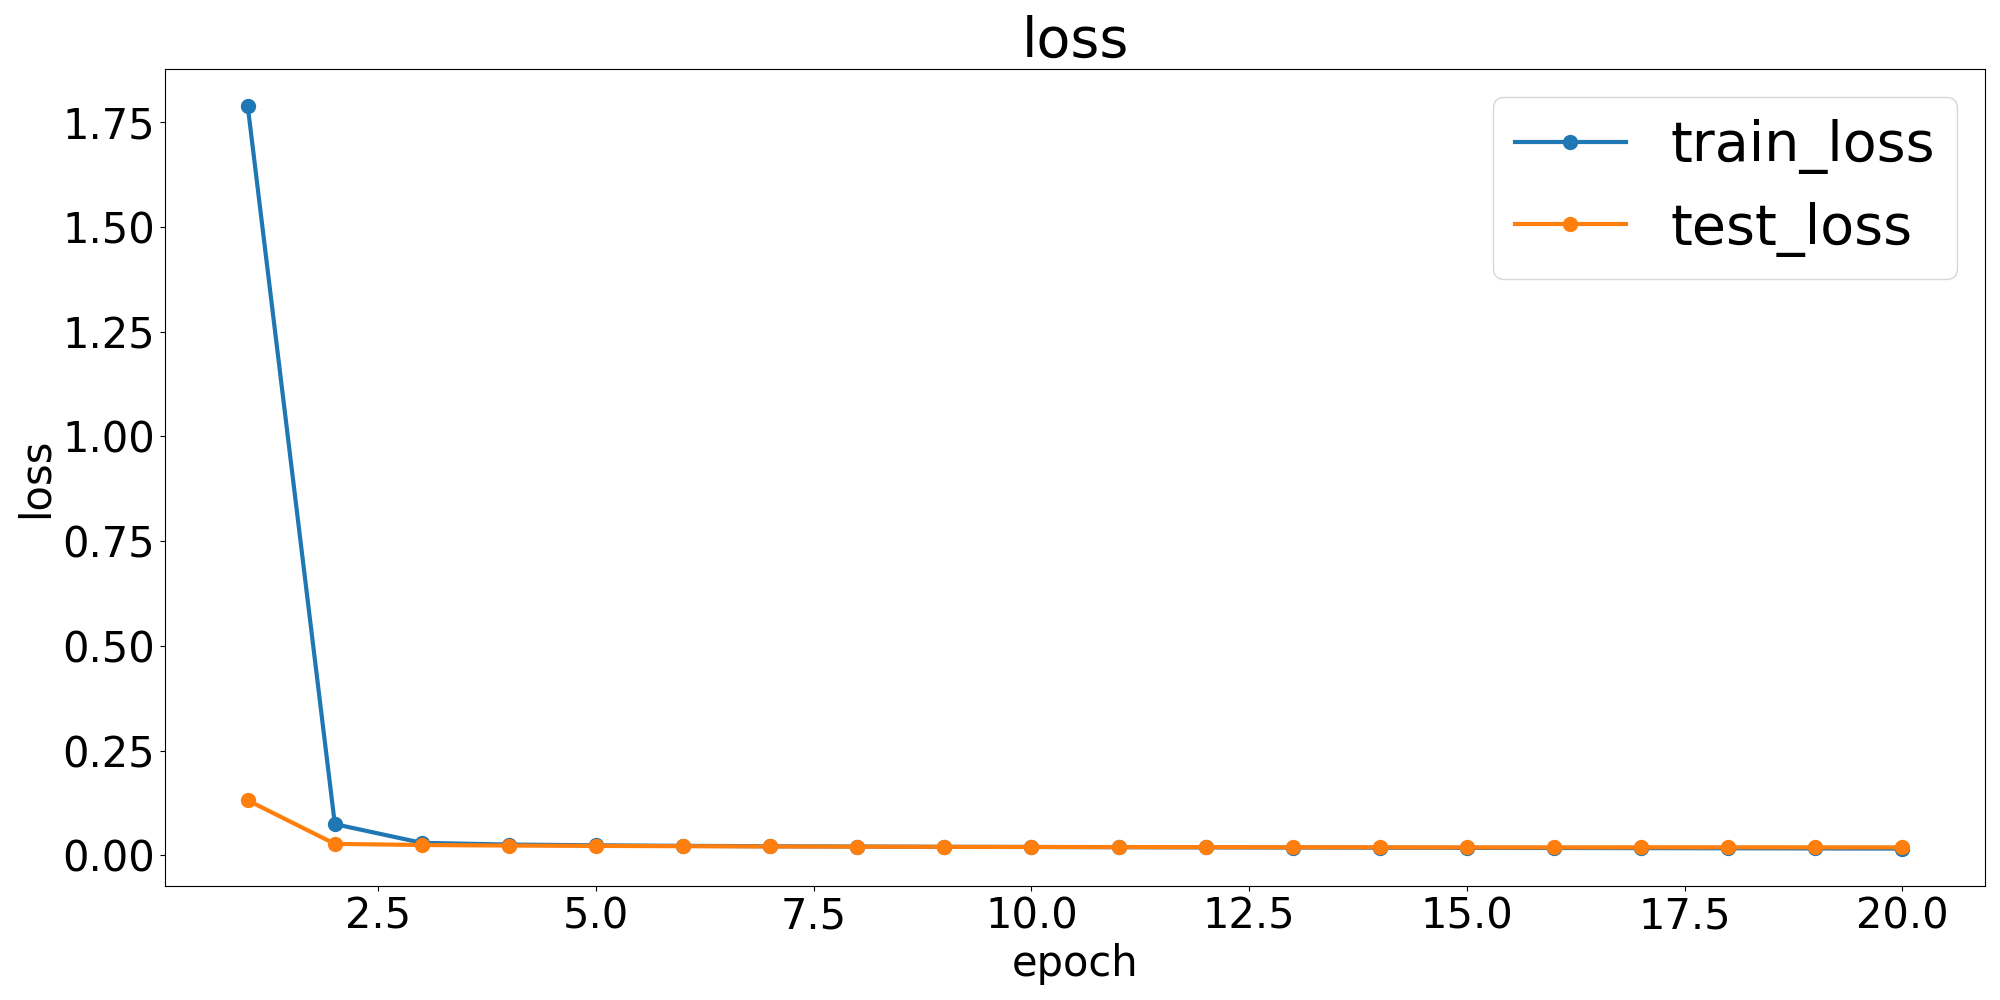
\includegraphics[width=\textwidth]{img/4-1.png}
    \end{subfigure}
    \hfill
    \begin{subfigure}[t]{0.45\linewidth}
        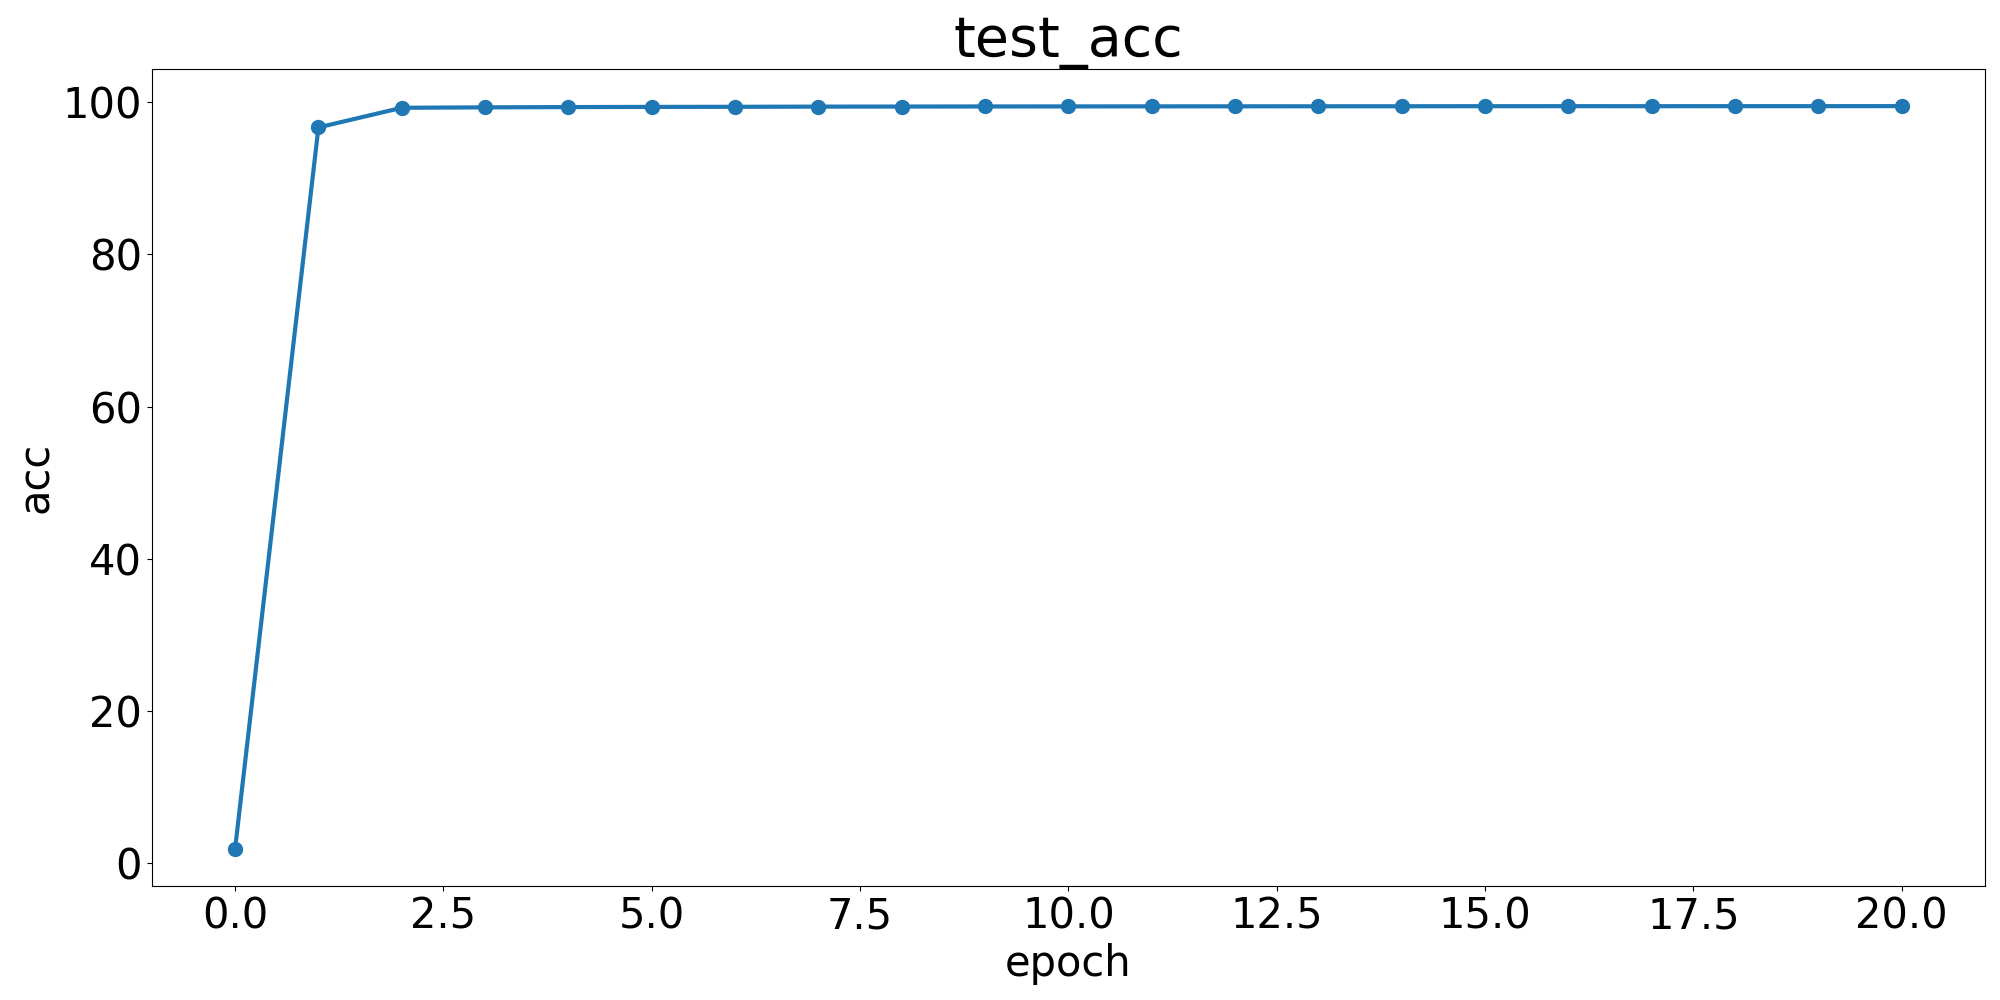
\includegraphics[width=\textwidth]{img/4-2.png}
    \end{subfigure}
    \hfill
\end{figure}


分析positional encoding的作用:

positional encoding通过给每一个词向量添加一部分与位置有关的信息,能够让词向量携带单词在序列中所处位置的信息,从而提高模型对序列的理解能力。


\section{有pos enc、有attn mask的Transformer}
训练结果:
\begin{figure}[H]
    \hfill
    \begin{subfigure}[t]{0.45\linewidth}
        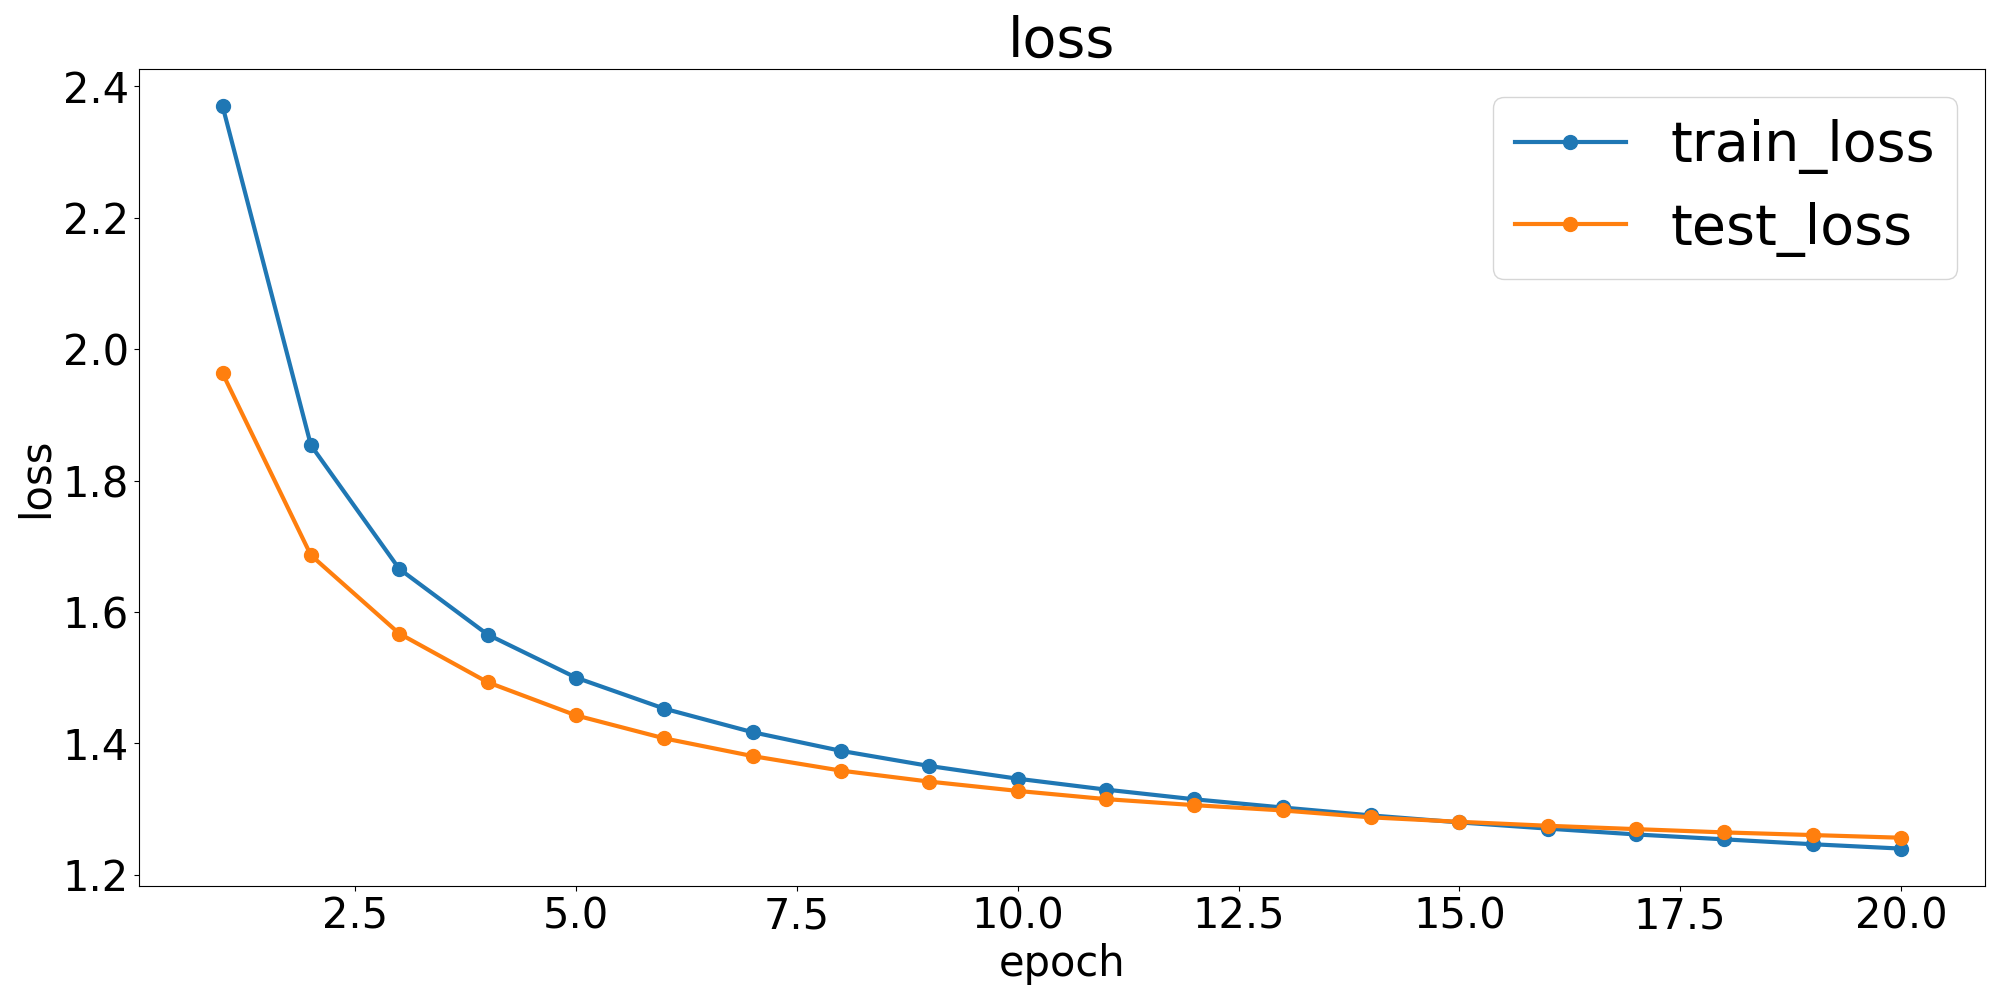
\includegraphics[width=\textwidth]{img/5-1.png}
    \end{subfigure}
    \hfill
    \begin{subfigure}[t]{0.45\linewidth}
        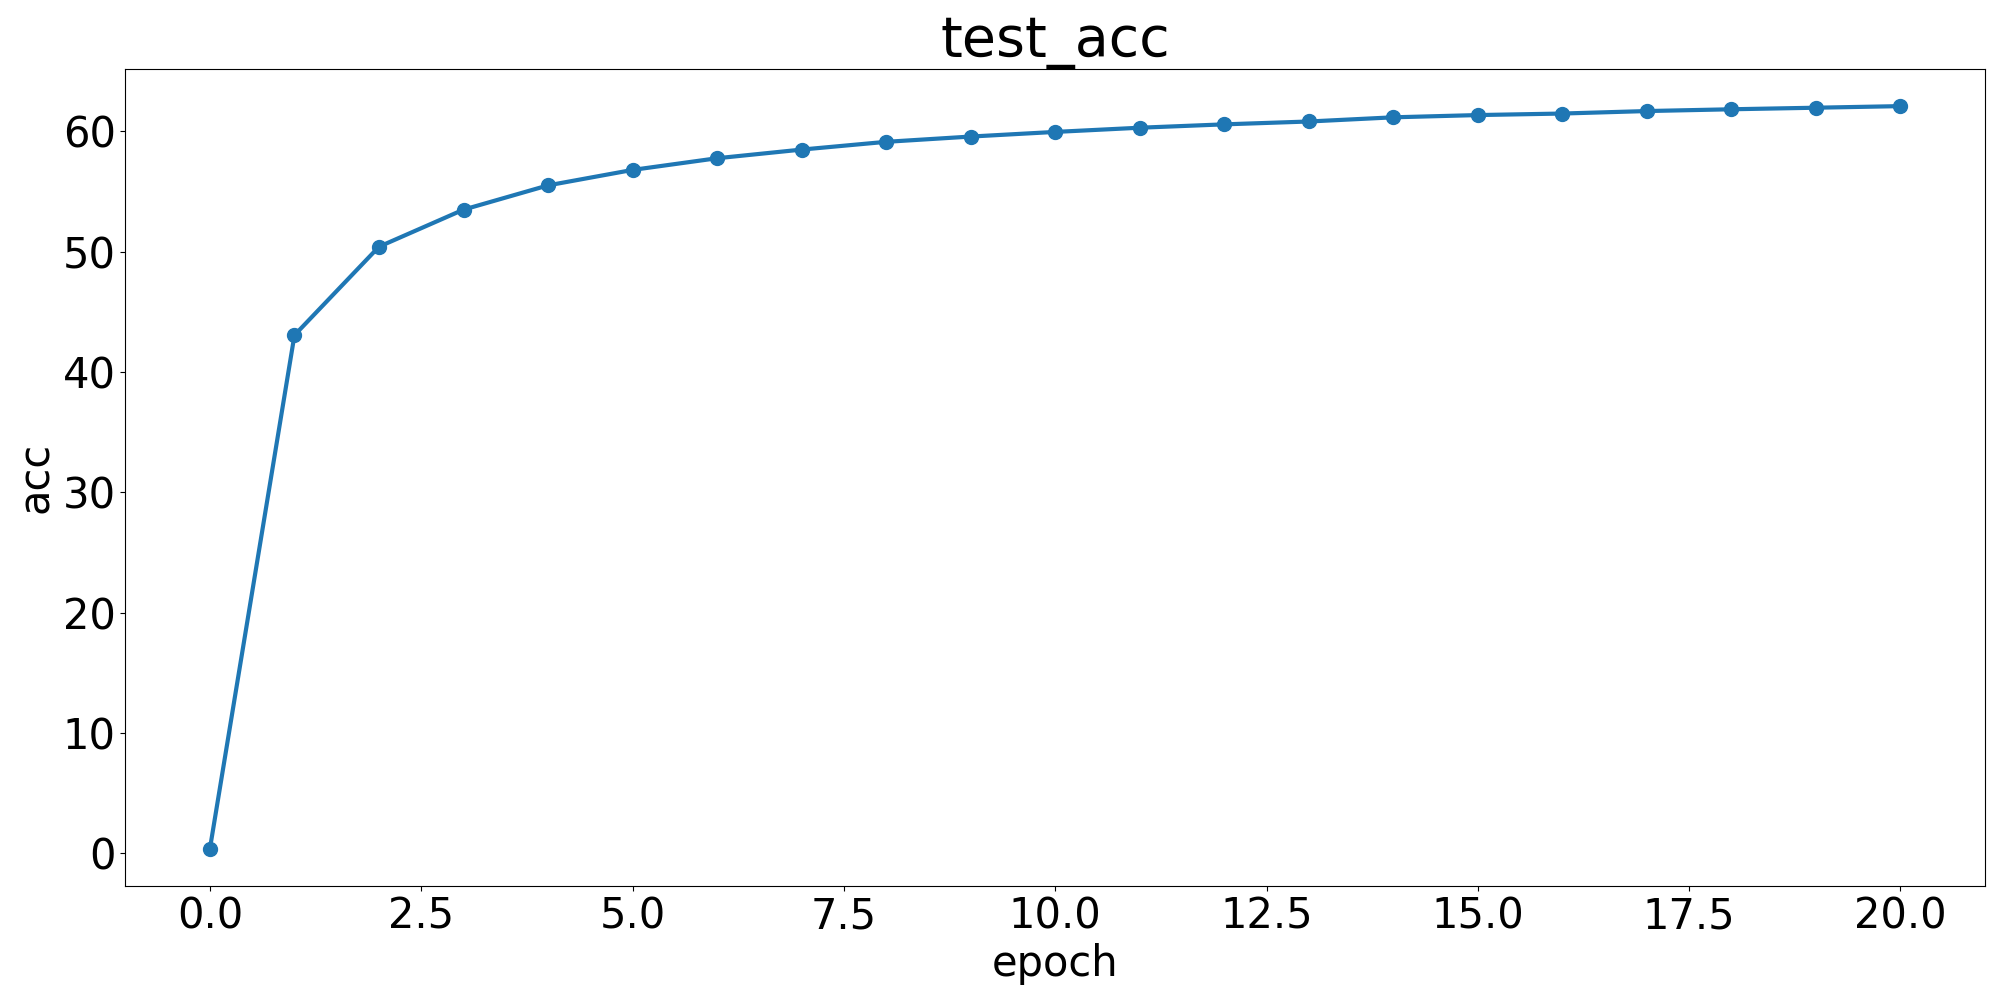
\includegraphics[width=\textwidth]{img/5-2.png}
    \end{subfigure}
    \hfill
\end{figure}


分析attention mask的作用:

attention mask能够确定有效token的位置,即屏蔽掉词向量中不需要模型关注的部分(比如只看当前词语左侧序列,屏蔽右侧序列),从而提高模型的性能和准确性。

\section{默认参数生成}
生成结果片段:
\begin{lstlisting}
Harry Potter saw he hurried out the end of the recently, starting (a shame to what they both to Skept throw that I was pulling him. Yes, you know that this is normal silent the sources Cedric of Magic is as his feath-magi was back on the ran towards the marble's already little sechoing from Leegn and his pratical elege. 
\end{lstlisting}

完整结果实例见附录。

\section{不同trategy和不同temperatures下生成内容的不同}
\begin{enumerate}
    \item 更改|strategy|为|'greedy'|

    生成结果片段:
\begin{lstlisting}
Harry Potter was a lot of the staff table and started to the staff table and started to the staff table and the staff table and the staff table and the staff table and the staff table and the staff table and the staff table and the staff table and the staff table and the staff table and the staff table
\end{lstlisting}

    由此可见,如果按greedy策略——每次都将下一个token选定为模型inference出的概率最大的那个,会导致输出结果随机性过小,产生单词不断循环重复的文本。

    完整结果实例见附录。

    \item 更改|temperature|
    
    生成结果片段:
    
    (|seed_words = "Harry Potter ",strategy = 'sampling'|)
\begin{lstlisting}
temperature = 0.0
    Harry Potter  embarrassed the school mustled by its of the forest changed so large particularly sleading being round his head soul of trouble enough. . . . . three you that lived out to life him back." "Harry?" sneered Ron, and Hermione," said Nick brandy suddenly. 

temperature = 0.5
    Harry Potter has been slid as where he did not supposed to himself's clear that he was Malfoy, as he did. . . . He got up this thing, Hagrid, excellently, howling floods to fake him his definitely as they left more were a loud. 

temperature = 2.0
    "So they heard Mr. Weasley almost interesting before he rupted it at more dead, Hermione," said Dumbledore, who paged the sixth the entrance fell we at Malfoy would have been here the only glasses, staring them as this missed students!" 

temperature = 5.0
    "Don't ter go anything I think we back to stand," said Harry,  after a little sense in his detrictical with the large across her plast, very conversation in a who sparks and the only Narcisss Entered,

temperature = 10.0
    "So. . een!' 'Cauld 'I suppose he attempt to a cast, when he had something turned on his feret about Hagrid when Dudley as he caught Slughorn was like your and dad into action.
\end{lstlisting}

    完整结果实例见附录。

    由以上生成结果可知,|temperature|越高,生成内容里出现错误单词的频率也越高,内容与句法也都不太连贯;而|temperature|较低时,虽然内容和句法仍旧很奇怪,但生成内容里很少出现错误单词。这是由于|temperature|越高,模型|inference|过程中输入到|softmax|函数的logit向量各值之间的差异就越小(|x = softmax(x / temperature)|),导致模型以|softmax|结果为pdf采样的时候采到最佳结果以外的样值的概率变大,使得模型最终生成结果准确率降低、但多样性提升。

\end{enumerate}


\section*{附:完整生成结果例}
一些完整生成结果实例如下:
\lstinputlisting{output/6.txt}
\lstinputlisting{output/7-1.txt}
\lstinputlisting{output/7-2.txt}

\end{document}